%%
%% Beuth Hochschule für Technik --  RCP Abschlussarbeit
%%
%% Hauptdokument
%%
%% 
%%
%%%%%%%%%%%%%%%%%%%%%%%%%%%%%%%%%%%%%%%%%%%%%%%%%%%%%%%%%%%%%%%%%%%%%
\documentclass[11pt, a4paper,parskip=half]{article}
%% Übersetzen als Entwurf
%\usepackage[entwurf]{bhtThesis}
%% Übersetzen für die Abgabe
\usepackage[abgabe]{bhtThesis}
\typeout{Deckblatt}

%\usepackage{float} %benutze ich für das richtige setzen der Bilder
\usepackage{blindtext}   %für Blindtext in Kapitel 2
\usepackage{listings}
\usepackage{color}
\lstset{ 
  literate={ö}{{\"o}}1
           {ä}{{\"a}}1
           {ü}{{\"u}}1
           {Ö}{{\"O}}1
           {Ä}{{\"A}}1
           {Ü}{{\"U}}1
           {ß}{{\ss}}1
}


\usepackage{trsym}
\usepackage{bytefield}
\definecolor{light-gray}{gray}{0.90} %Code Hintergrundfarbe

\usepackage{longtable}

%%
%% Pfad zu den Bildern
%%
\graphicspath{
  {pictures/},
  {einleitung/pictures},
  {kapitel1/pictures/},
  {kapitel2/pictures/},
  {kapitel3/pictures/},
  {kapitel4/pictures/},
  {kapitel5/pictures/},
  {kapitel6/pictures/},
  {kapitel7/pictures/},
  {kapitel8/pictures/}
}

% julians einstellungen
\definecolor{darkBHT}{rgb}{0,0.5882,0.5529}
\setlength{\parskip}{6pt} 
\setlength{\parindent}{0pt}

\definecolor{lightgray}{rgb}{.9,.9,.9}
\definecolor{darkgray}{rgb}{.4,.4,.4}
\definecolor{purple}{rgb}{0.65, 0.12, 0.82}

\lstdefinelanguage{JavaScript}{
  keywords={typeof, new, true, false, catch, function, return, null, catch, switch, var, if, in, while, do, else, case, break},
  keywordstyle=\color{blue}\bfseries,
  ndkeywords={class, export, boolean, throw, implements, import, this},
  ndkeywordstyle=\color{darkgray}\bfseries,
  identifierstyle=\color{black},
  sensitive=false,
  comment=[l]{//},
  morecomment=[s]{/*}{*/},
  commentstyle=\color{purple}\ttfamily,
  stringstyle=\color{red}\ttfamily,
  morestring=[b]',
  morestring=[b]"
}

\begin{document}
\pagestyle{fancy}


% \maketitle %Deckblatt


\begin{titlepage}
	\begin{center}
		\Large
		Beuth Hochschule für Technik Berlin
		\textcolor{darkBHT}{\rule{\textwidth}{0.2cm}} \\
		\vspace{2 cm}
		
		
		\begin{figure}[htbp]
			\centering 
			
\includegraphics[width=9cm]{BHT-Logo-Basis.pdf}  
		\end{figure}
		
		\vspace{1cm}
		
		\Large
		Fachbereich VI - Technische Informatik - Embedded Systems\\
		Fach Rapid Control Prototyping\\
		SS 2014\\
		\vspace{2 cm}
		
		\Huge
		\textbf{Regelung einer simulierten Druckregelstrecke (II)}
		\vspace{2 cm}
	
		\Large
		Eingereicht am \\
		\today % Aktuelles Datum
		\vspace{0.8cm}
		
		Eingereicht von \\
		\begin{tabular}{ll}
			Matthias Hansert & s791744\\
			Marcus Perkowski & s798936\\
			Marcel Burde & s798984\\
		\end{tabular}

	\end{center}
	\vfill
	\textcolor{darkBHT}{\rule{\textwidth}{0.2cm}}
	\vspace{1 cm}
	\normalsize
	
\end{titlepage}

%
% EOF
%


\pagenumbering{roman}
%%%%%%%%%%%%%%%%%%%%%%%%%%%%%%%%%%%%%%%%%%%%%%%%%%%%%%
%%%%%%%%%%%%%%%%%%%%%%%%%%%%%%%%%%%%%%%%%%%%%%%%%%%%%%

\newpage
\begin{huge}
Aufgabenstellung\\

\end{huge}
Entwerfen und optimieren Sie einen Regelkreis, der den Arbeitspunktdruck für alle möglichen Belastungsfälle (Schalter "ein" und anschließend Schalter "aus") möglichst schnell und ohne Übersteuerung der Stellgröße ausregelt und stationär konstant hält.\\

Berücksichtigen Sie dabei, dass primär Störungen ausgeregelt werden sollen. Eine Führung des Kreises in den Arbeitspunkt erfolgt nur nach Inbetriebnahme der Strecke (ca. 1 mal pro Woche).\\

Nehmen Sie (bis auf das Einstecken der notwendigen Kabelanschlüsse und die Betätigung des Störschalters) keine Änderungen (z.B. Veränderung von Potentiometereinstellungen) am Simulationsgerät vor.\\

Das Simulationserät simuliert einen elektrisch steuerbaren hydraulischen Druckgenerator für den Antrieb einer Arbeitsmaschine. Die Anschlußkonfiguration der Eingangs- und Ausgangssignale ist auf dem folgenden Bild (nächste Seite ) dargestellt:\\

\begin{itemize}
\item Mittels einer Steuerspannung u(t), die einen Aussteuerbereich von -10V bis 10V hat, aber nur im positiven Bereich genutzt werden soll, kann der Druck zwischen 0 und einem Maximalwert verstellt werden.

\item $y_{M} (t)$, die Meßgröße des erzeugten Drucks, kann auf der rechten Seite der Anordnung an einer Buchse in Form einer elektrischen Spannung gemessen werden. Die Meßeinrichtung arbeitet linear und der Verstärkungsfaktor beträgt $V =0,08 \dfrac{V}{Bar}$.\\
Die Meßeinrichtung habe PT1-Verhalten, wobei ihre Zeitkonstante klein gegen die der Strecke ist, so daß sie vernachlässigt werden kann.

\end{itemize}


Der Generator arbeitet mit einem Arbeitspunktdruck von 50 Bar bei einer Grundlast, die anliegt, wenn der „Störschalter“ in der Stellung ohne Beschriftung (also nach unten) steht. Durch eine Schalterbewegung in Richtung „ein“ (nach oben) kann eine maximale Entlastung des Druckgenerators simuliert werden.


\begin{figure}[htbp]
	\begin{center}
		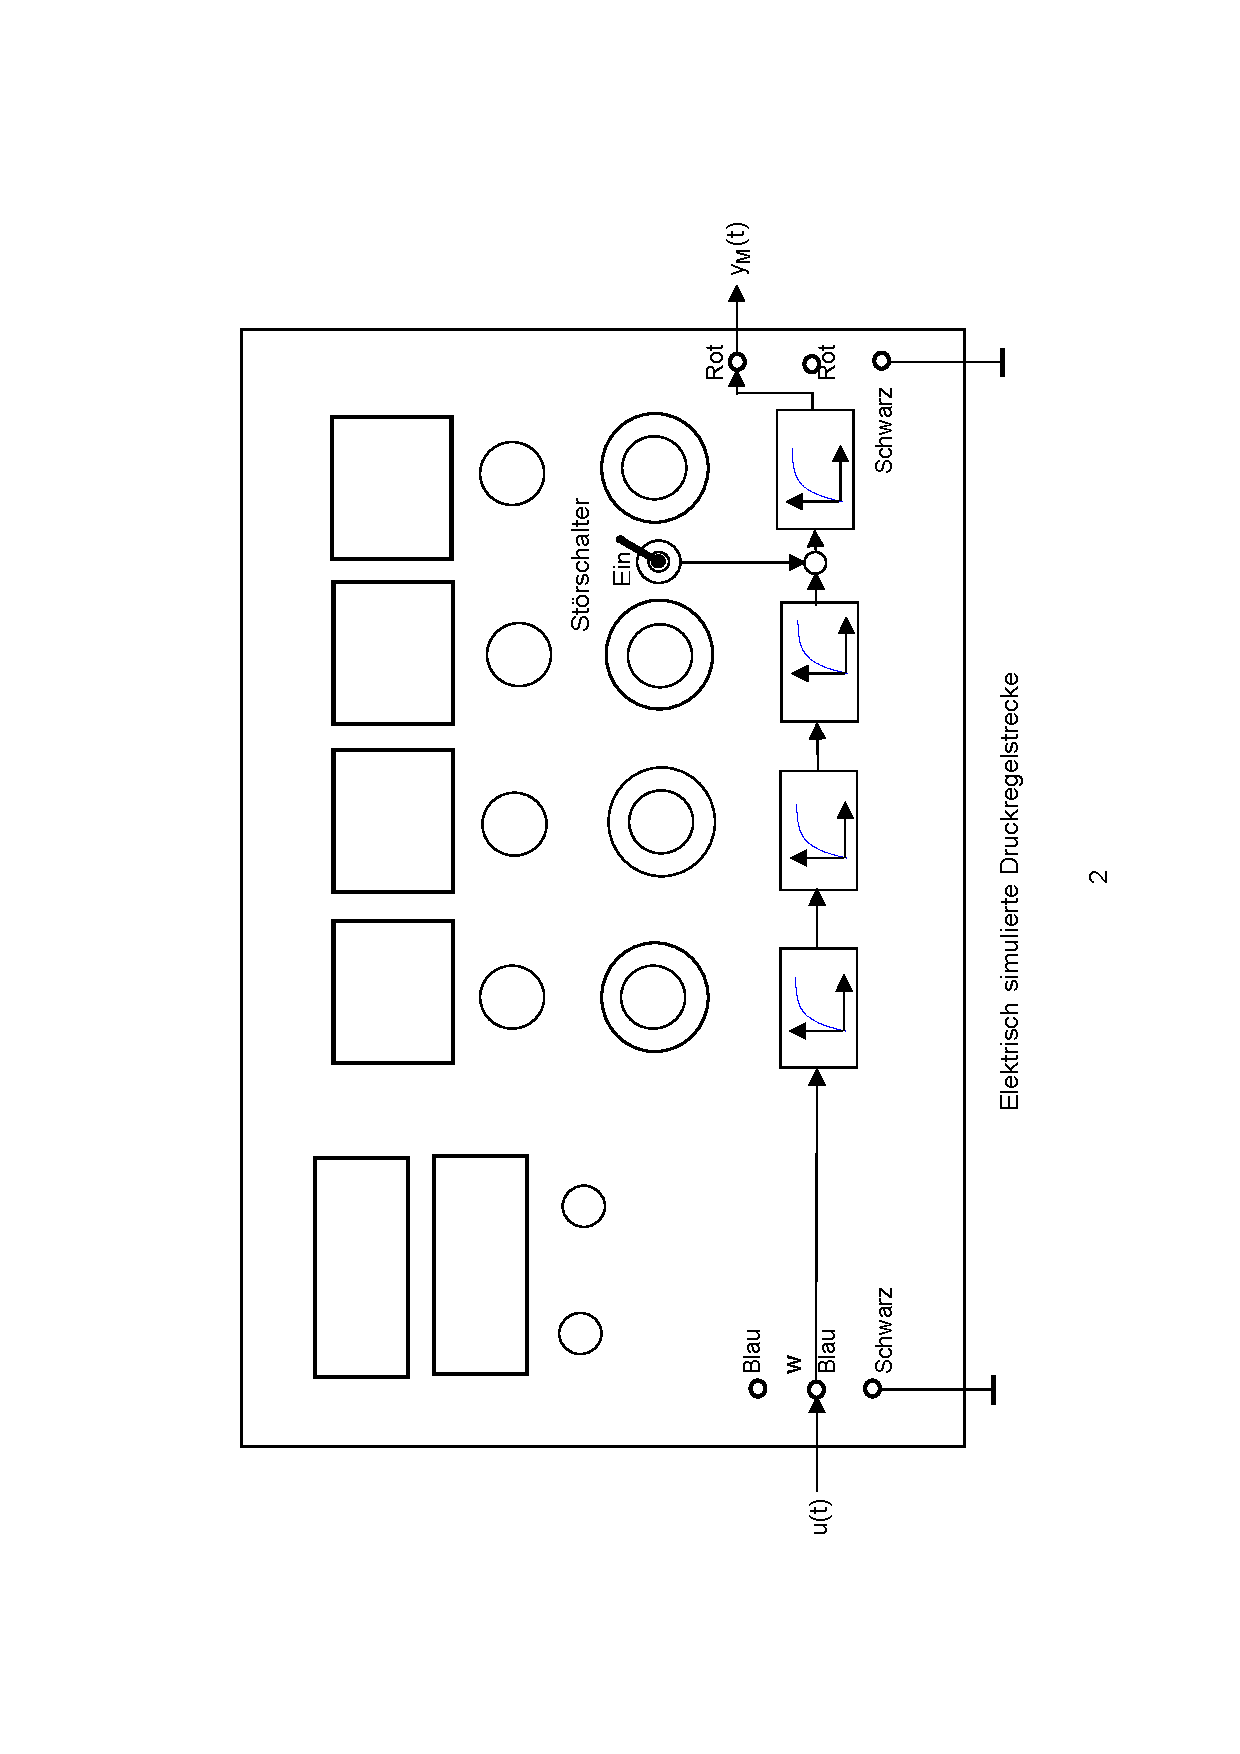
\includegraphics[width=15cm]{elektrischeSchaltung.pdf} 
	\end{center} 
\end{figure}


%%%%%%%%%%%%%%%%%%%%%%%%%%%%%%%%%%%%%%%%%%%%%%%%%%
%%%%%%%%%%%%%%%%%%%%%%%%%%%%%%%%%%%%%%%%%%%%%%%%%%
\newpage
\begin{huge}
Auflistung aller abgegebenen Dateien\\

\end{huge}

\begin{itemize}
\item \textbf{01\_Vorbereitung}
	\begin{itemize}
	\item first item
	\end{itemize}
	
\item \textbf{02\_Statische\_Kennlinie}
	\begin{itemize}
	\item first item
	\end{itemize}
	
\item \textbf{03\_Steuerverhalten\_Strecke}
	\begin{itemize}
	\item first item
	\end{itemize}
	
\item \textbf{04\_Stoerverhalten\_Strecke}
	\begin{itemize}
	\item first item
	\end{itemize}
	
\item \textbf{05\_Simulation\_Strecke}
	\begin{itemize}
	\item first item
	\end{itemize}
	
\item \textbf{06\_Reglerentwurf}
	\begin{itemize}
	\item first item
	\end{itemize}
	
\item \textbf{07\_Simulation\_Regelkreis}
	\begin{itemize}
	\item first item
	\end{itemize}
	
\item \textbf{08\_Regler\_Reale\_Strecke}
	\begin{itemize}
	\item first item
	\end{itemize}
	
\item \textbf{09\_Sonstiges}
	\begin{itemize}
	\item Vorgehensweise\_zur\_Erstellung\_Belegarbeit
	\item Labor-Übung 11 (Simulierte Druckregelstrecke\_2)
	\end{itemize}
	
\item \textbf{10\_Hilfsprogramme}
	\begin{itemize}
	\item polkomp.m
	\item sys\_id
	\item tf2vn.m
	\end{itemize}

\end{itemize}



%%%%%%%%%%%%%%%%%%%%%%%%%%%%%%%%%%%%%%%%%%%%%%%%%%%%%%
%%%%%%%%%%%%%%%%%%%%%%%%%%%%%%%%%%%%%%%%%%%%%%%%%%%%%%


\newpage
\tableofcontents %Inhaltsverzeichnis


\pagenumbering{arabic}
%%%%%%%%%%%%%%%%%%%%%%%%%%%%%%%%%%%%%%%%%%%%%%%%%%%%%%%%%%%%%%%
%% Die Kapitel der Arbeitw
%%
%% Beuth Hochschule für Technik 
%%
%% Einleitung 1
%%
%%

\newpage
\section{Zu regelndes Objekt kennen lernen}
Das Objekt was wir regeln sollen handelt sich um einen elektrischen steuerbaren hydraulischen Druckgenerator für den Antrieb einer Arbeitsmaschine. Zu beachten ist das es sich um eine simulierte Druckregelstrecke handelt.\\

Bekannt ist:
\begin{itemize}
\item Steuerspannung -10V $\leq u(t) \leq$ 10V, wobei nur der positive Bereich betrachtet wird, weil der Druck von 0 bis einem Maximalwert verstellt wird

\item Die Messgröße $Y_{M}(t)$ wird in Form einer Spannung gemessen

\item Der Verstärkungsfaktor der Messeinrichtung $V_{M}$ beträgt $0,08\frac{V}{Bar}$

\item Bei einer Grundlast liegt der Arbeitspunktdruck bei 50 Bar

\item Die Messeinrichtung hat ein PT1-Verhalten wo die Zeitkonstante vernachlässigt werden kann 
\end{itemize}


Wenn man das Objekt (Abbildung \ref{RegelKreis}) genauer betrachtet, können die Teile eines Standard-Regelkreises erkannt werden:
\begin{itemize}
\item $u(t)$ Regelgröße
\item $y(t)$ Stellgröße
\item Stelleinrichtung und Regelstrecke
\end{itemize}

\begin{figure}[htbp]
	\begin{center}
		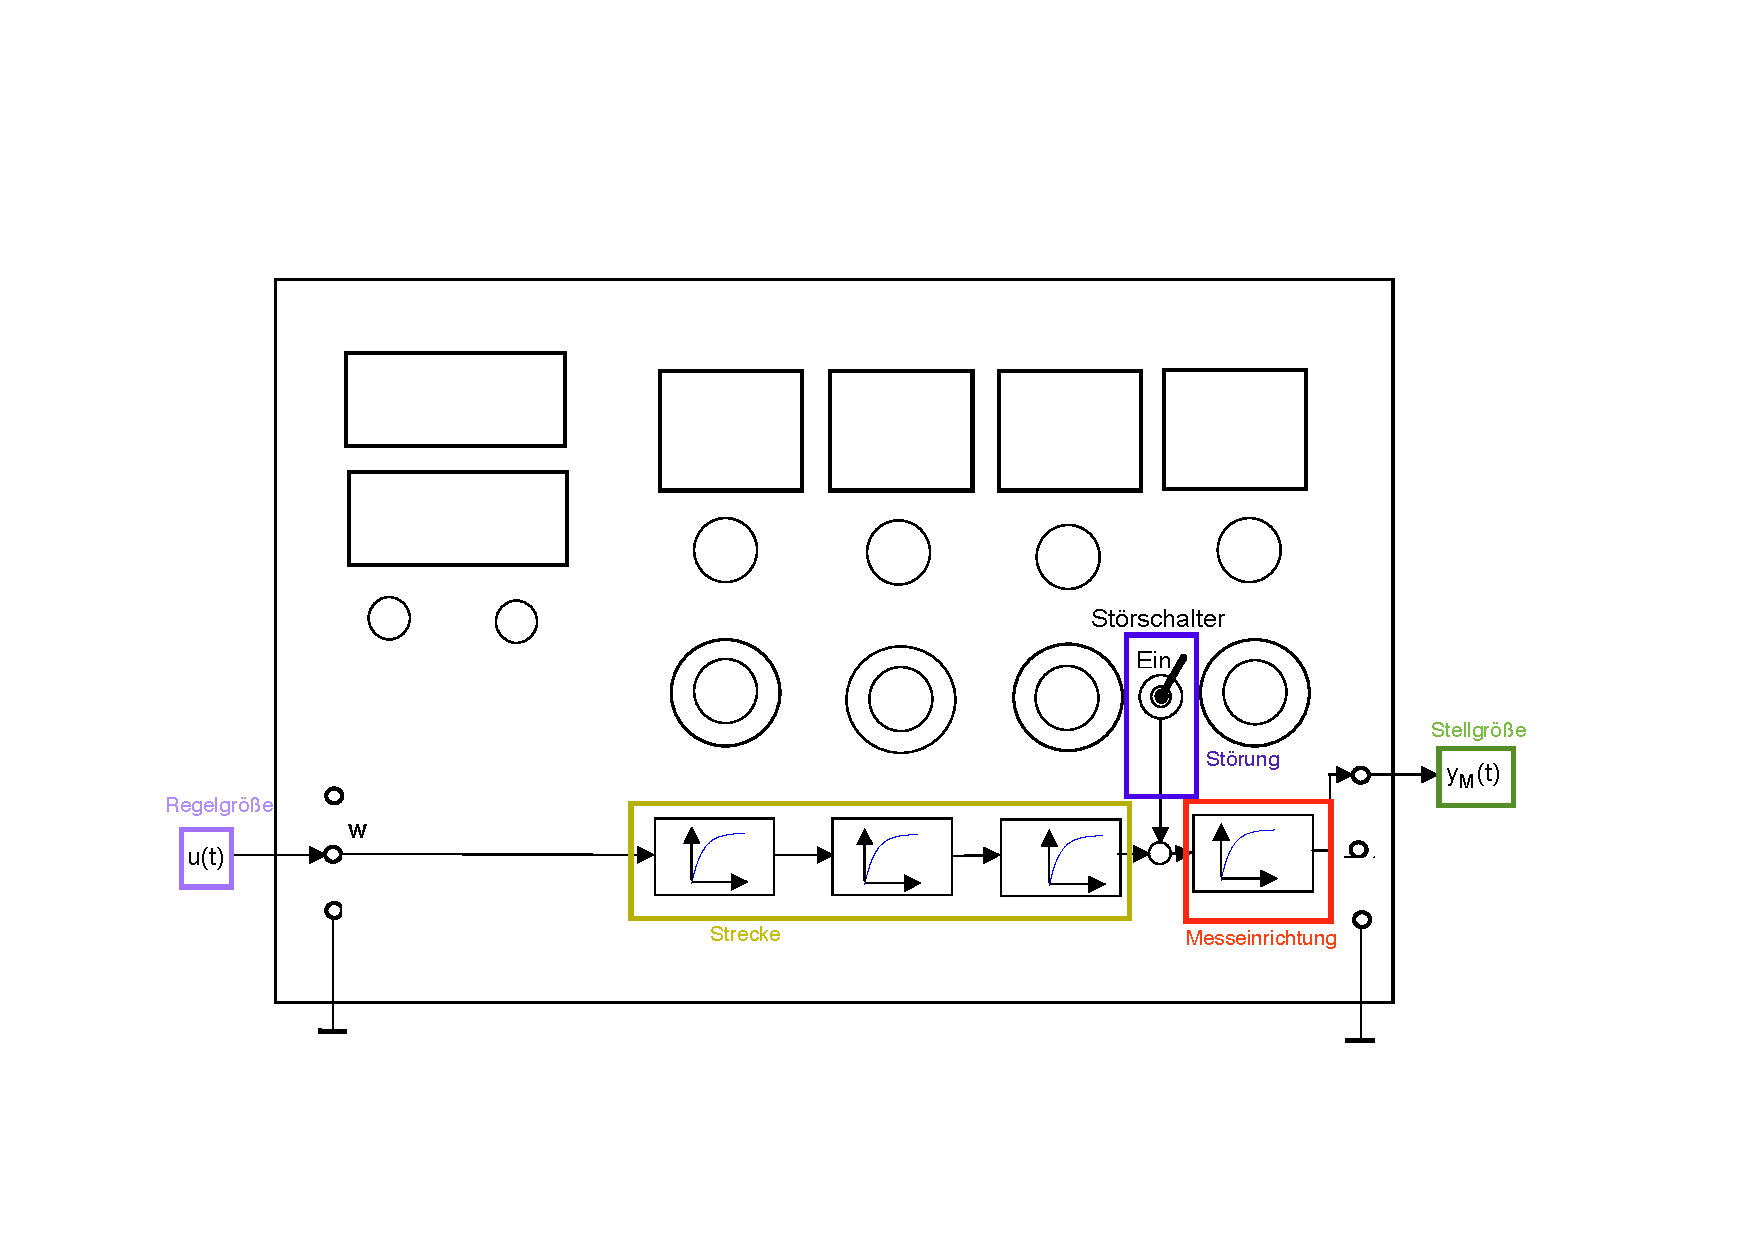
\includegraphics[scale=0.4]{regelkreis.pdf}
		\caption{Elektrische simulierte Druckregelstrecke mit Standard-Regelkreis}
       \label{RegelKreis}
	\end{center} 
\end{figure}

\newpage

Um alle Größen zu bestimmen/messen und der Reger zu entwickeln wird MATLAB/Simulink eingesetzt. Dies geschieht mit das Tool Real-Time-Workshop und eine A/D-D/A Wandlerkarte.


\subsection{Offset}
Um das System mit dem Rechner zu verbinden wird eine Wandlerkarte eingesetzt. Die Wandlerkarte ist im PC eingebaut. Um Fälschungen im Ergebnis zu umgehen muss der Eingang- und Ausgangsoffset gemessen werden. Um diese Werte zu messen wurde das \textit{reinraus2007b.mdl} Simulinkmodell benutzt.\\

Für den Eingangsoffset der Wandlerkarte wurde ein Display 



%Für das bestimmen der Offsetwerte haben wir das reinraus2007b.mdl Simulinkmodell benutzt. Bei dem Input wurde ein Display als Offset-Ausgabe benutzt und der entsprechende Gegenoffset über einen Summenpunkt addiert oder subtrahiert. Wichtig hier ist das man die beiden Leitungen die von der Wandlerkarte zur simulierten Druckeregelstrecke gehen miteinander kurz schließt. Für den Output müssen die zwei Leitungen an ein Messgerät angeschlossen werden, dies dann den vorhandenen Offset anzeigt. Im Simulinkmodell wird, wie für den Input, dann der Gegenoffset addiert oder subtrahiert.

%%%%%%%%%%%%%%%%%%%%%%%%%%
%% bild einfügen

%\begin{figure}[h]
%	\begin{center}
%		\includegraphics[scale=0.5]{pic.jpg}
%		\caption{bildbeschreibung - titel}
%       \label{für referenzen}
%	\end{center} 
%\end{figure} %

%%
%% Beuth Hochschule für Technik --  
%%
%% Kapitel 2 - 
%%
%%	

\newpage
[Hansert]
\section{Festlegung des Arbeitpunktes}

Laut Aufgabestellung liegt der Arbeitspunktdruck bei einer Grundlast bei $50Bar$. Da unser System einen Spannungsbereich von 0 bis $10V$ besitzt, müssen wir den Druck in eine Spannung übersetzen.

$Arbeitspunkt = Arbeitspunktdruck * Verstaerkung$\\
$Arbeitspunkt = 50Bar * 0,08V/Bar$\\
$Arbeitspunkt = 4V$\\ 


Um den Arbeitspunkt zu ermitteln muss zuerst das Verhalten des Systems festgestellt werden.


\subsection{Statisches Verhalten}
Um die Kennlinie des Systems zu ermitteln wird, mithilfe des Simulinkmodells \textit{Statische\_Kennlinie.mdl}, eine sprungförmige Erregung mit 20 Schritten, bei jedem Schritt $t= sek$ die Spannung um $0,5V$ erhöht. $t$ wurde so gewählt dass das System einen stationären Zustand erreicht, bevor es neu angeregt wird (Siehe Abbildung \ref{ScopOut} und \ref{ScopIn}).

\begin{figure}[h]
	\begin{center}
		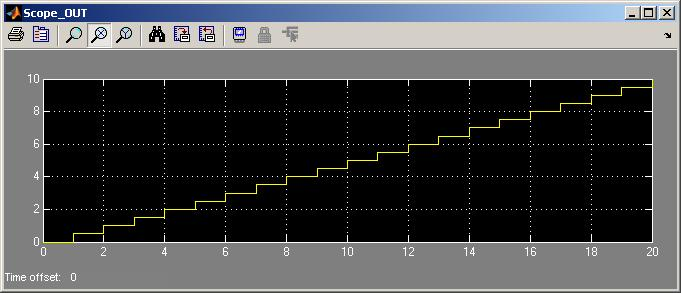
\includegraphics[scale=0.5]{scope_out.jpg}
		\caption{Ausgangssignal, Erregung des Systems}
       \label{ScopOut}
	\end{center} 
\end{figure}


\begin{figure}[h]
	\begin{center}
		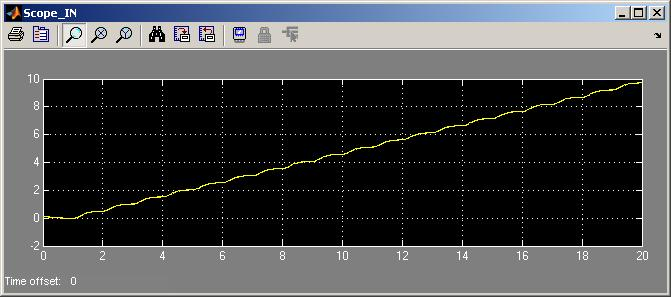
\includegraphics[scale=0.5]{scope_in.jpg}
		\caption{Eingangssignal, Antwort des Systems}
       \label{ScopIn}
	\end{center} 
\end{figure}

Die Antwort wird in der Matrix \textit{ScopeIn.mat} gespeichert und mit dem MATLAB Script \textit{Berechnung\_Kennlinie.m} wird die statische Kennlinie berechnet und gezeichnet (siehe Abbildung \ref{StatKenn}). Um Fehler zu vermeiden haben wir uns dazu entschieden einen Durchschnittswert zu berechnen, dieser besteht aus 20 Werten bevor das System neu erregt wird.


\begin{figure}[h]
	\begin{center}
		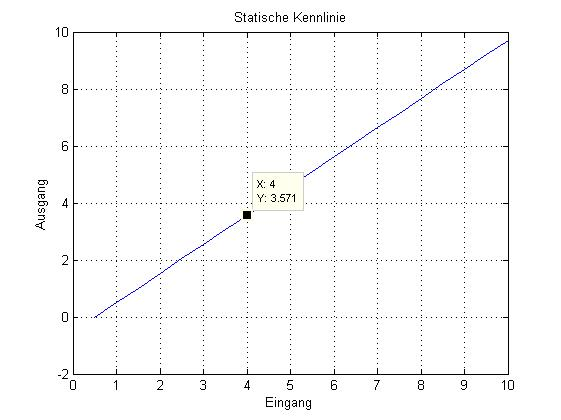
\includegraphics[scale=0.5]{arbeitspunkt.jpg}
		\caption{Statische Kennlinie, Ausgang $y(t)/V$, Eingang $u(t)/V$}
       \label{StatKenn}
	\end{center} 
\end{figure}

In der Abbildung \ref{StatKenn} ist deutlich zu erkennen, dass es sich um eine lineares System handelt, da die Verstärkung konstant bleibt. %
%%
%% Beuth Hochschule für Technik --  
%%
%% Kapitel 3 -
%%
%%	

\newpage

\section{section33}
 %
%%
%% Beuth Hochschule für Technik --  
%%
%% Kapitel 4 - 
%%
%%	

\newpage
[Perkowski]
\section{Messtechnische Identifikation des Störverhaltens der Strecke}
Da das Verhalten der Störübertragungsfunktion zu ermitteln ist, kann wie im Kapitel 3 durchgeführt werden. Die Strecke wird erst in den Arbeitspunkt erregt und dann die Störgröße mit einem Schalter an der Hardware zugeschaltet. Wir haben die Störmessung aufgezeichnet \textit{(stoer\_err.mat)}.

\begin{figure}[h]
	\begin{center}
		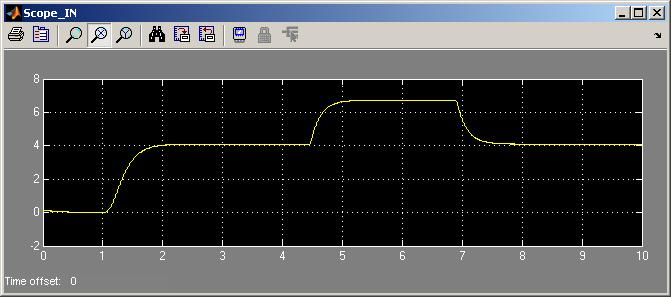
\includegraphics[scale=0.5]{stoerung.jpg}
		\caption{Strecke mit Störung}
       \label{stoer}
	\end{center} 
\end{figure}

Nachdem wir die gemessene Sprungantwort betrachten, sind wir aufgrund des typischen Verhaltens ausgegangen, dass es sich um PT1-System handelt. 
Da mit Hilfe des Tools \textit{sys\_id} die Zeitachse der Störung eingegrenzt werden kann, kann an dieser Stelle die Identifikation der Störstrecke durchgeführt werden. Das Ergebnis kann im folgenden Bild nachvollzogen werden.

Die ermittelte Störungsfunktion:

\begin{center}
$ G(s)_{stoer} = \dfrac{2,6424}{1 + 0,16207} $
\end{center}

\begin{figure}[h]
	\begin{center}
		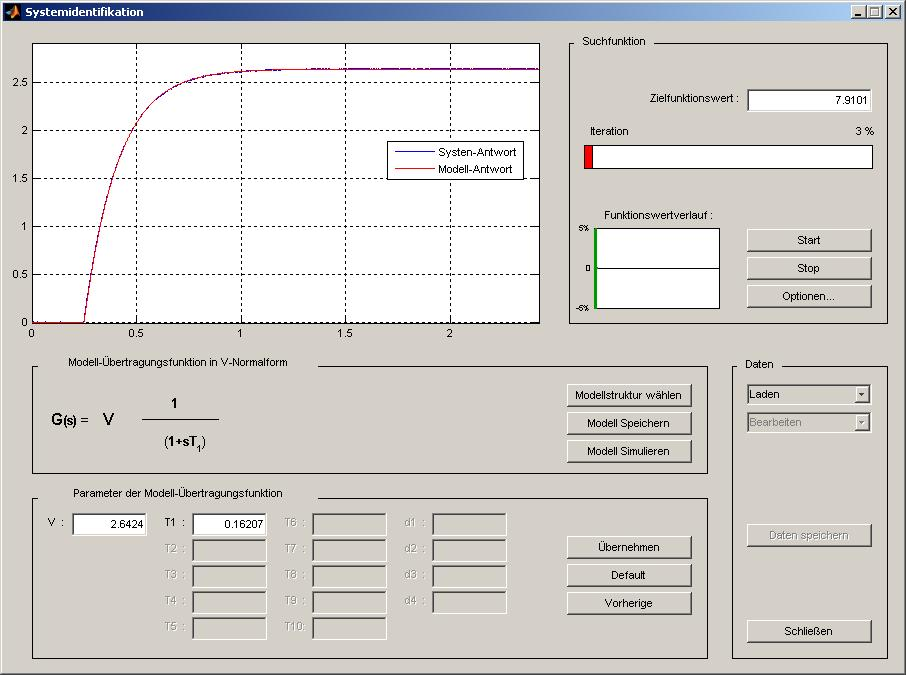
\includegraphics[scale=0.5]{stoerung_1_uebfkt.jpg}
		\caption{erster Ausschnitt Übertraungsfunktion mit Störung}
       \label{stoerfkt1}
	\end{center} 
\end{figure}

\begin{figure}[h]
	\begin{center}
		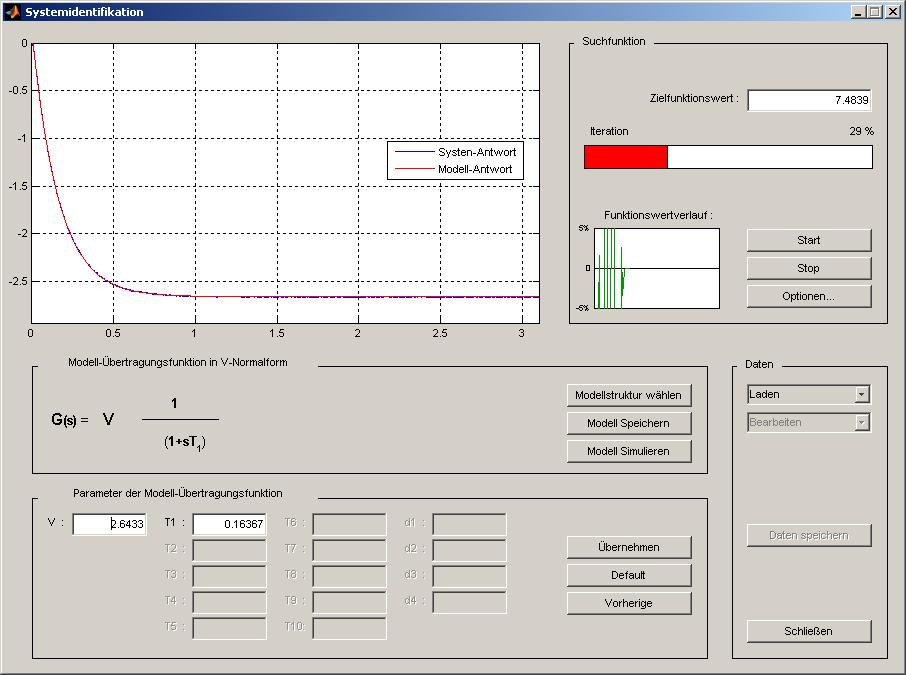
\includegraphics[scale=0.5]{stoerung_2_uebfkt.jpg}
		\caption{zweiter Ausschnitt Übertraungsfunktion mit Störung}
       \label{stoerfkt2}
	\end{center} 
\end{figure}

 %
%%
%% Beuth Hochschule für Technik --  
%%
%% Kapitel 5 - 
%%
%%	

\newpage


\section{section55} %
%%
%% Beuth Hochschule für Technik --  
%%
%% Kapitel 6 - 
%%
%%	

\newpage

[Burde]

\section{Entwurf des Reglers}

Nachdem nun die Strecke zunächst identifiziert und anschließend das Steuer- und Störverhalten simuliert wurde, soll nun der passende Regler entworfen werden. Der Regler hat dabei folgende Aufgaben: Er soll dafür sorgen, dass die Regelgeschwindigkeit des Regelkreises möglichst hoch wird und er soll bleibende Regelabweichungen verhindern, also eine hohe Regelgenauigkeit vorweisen.

Die Entscheidung fällt zunächst einmal auf einen PI-Regler. Der P-Anteil sorgt für eine hohe Regelgeschwindigkeit und kompensiert somit die Trägheit des I-Anteils. Gleichzeitig sorgt jedoch der I-Anteil dafür, dass die durch den P-Anteil entstehende bleibende Regelabweichung entfernt wird. 

Um den Verstärkungsfaktor V und die Reglerzeitkonstante T optimal bestimmen zu können, wird als Entwurfsverfahren das Polkompensationsverfahren gewählt. Wie der Name schon aussagt, lassen sich bei diesem Verfahren Verzögerungsglieder aus der Strecke bzw. Messeinrichtung durch eventuelle Vorhalteglieder aus dem gewählten Regler kompensieren. Verzögerungsglieder sorgen meist für ein langsameres Ausregeln von Störgrößen und sind daher unerwünscht. Die nachfolgenden Übertragungsfunktionen vom PI-Regler sowie von der Strecke zeigen das Vorhalteglied des Reglers, welches das markierte Verzögerungsglied der Strecke kompensieren soll. 

\begin{center}
$ G_{R}(s) = \dfrac{V*\textbf{(1+sT)}}{s} $
\end{center}

\begin{center}
$ G_{S}(s) = \dfrac{1,03}{(1 + 0,003365s) * \textbf{(1 + 0,1864s)} * (1 + 2*0,98029s + (0,091032s)^{2}) }$
\end{center}

Die Zählerzeitkonstante des PI-Reglers beträgt also $ T = 0,1864[sek] $. Um den Verstärkungsfaktor des Reglers zu bestimmen, muss nun das Bodediagramm des offenen Regelkreises gezeichnet werden. Da der Aufwand dafür recht hoch ist, haben wir die Polkompensation mit dem Matlab-Programm \textit{polkomp} durchgeführt.
 %
%%
%% Beuth Hochschule für Technik --  
%%
%% Kapitel 7 - 
%%
%%	

\newpage


\section{Simulation des Regelkreises mit dem entworfenen Regler}
 %
%%
%% Beuth Hochschule für Technik --  
%%
%% Kapitel 5 - 
%%
%%	

\newpage

[Burde]
\section{Implementierung des Reglers in den realen Regelkreis}

 %


%%%%%%%%%%%%%%%%%%%%%%%%%%%%%%%%%%%%%%%%%%%%%%%%%%%%%%%%%%%%%%%%
%Abbildungsverzeichnis
\newpage
\listoffigures
		
%\newpage
%\begin{appendix}
%  %%
%% Beuth Hochschule für Technik --  Abschlussarbeit
%%
%% Anhang
%%
%%%%%%%%%%%%%%%%%%%%%%%%%%%%%%%%%%%%%%%%%%%%%%%%%%%%%%%%%%%%%%%%%%%%%


\section{Anhang}



%\end{appendix}



%%%%%%%%%%%%%%%%%%%%%%%%%%%%%%%%%%%%%%%%%%%%%%%%%%%%%%%%%%%%%%%
%% Literaturverzeichnis

\clearpage
\newpage
\addcontentsline{toc}{section}{Literatur- und Quellenverzeichnis}
\nocite{*}
\bibliographystyle{IEEEtran}
\bibliography{bhtThesis}

\end{document}
